\documentclass[11pt]{article}

\usepackage[letterpaper,left=1.6in,right=1.6in,top=1.2in,bottom=1.2in]{geometry}

\usepackage[T1]{fontenc}
\usepackage[utf8]{inputenc}

\usepackage{lmodern}
\usepackage{amssymb,amsmath}
\usepackage{algorithm,algorithmic}
\usepackage{hyperref}
\usepackage{graphicx}
\usepackage{listings}
\usepackage[11pt]{moresize}

\setcounter{secnumdepth}{0}

%\usepackage[vlined]{algorithm2e}
\usepackage{algorithm,algorithmic}
\usepackage{paralist}
\usepackage{tikz}
\usepackage{xcolor,colortbl}

\begin{document}
\lstset{language=Java}
\begin{center}
\begin{HUGE}{\bf A6b - Shipping Game}\\ \end{HUGE}
\vspace{3mm}
\begin{LARGE} By Michael Patashnik and the CS2110 Course Staff\\ \end{LARGE}
\vspace{7mm}
\begin{LARGE} Contents\\ \end{LARGE}
\noindent\rule{8cm}{0.4pt}
\begin{enumerate} \begin{large}
\item Introduction\item Game overview
\item Installation and running
\item Using the GUI
\item Brief introduction to the classes
\item Your tasks
\item Concurrency
\item What to hand in when
\end{large}\end{enumerate}
\end{center}

\section{1. Introduction}
You can work on A6b in groups of two. Form the group well before the assignment due date. Both must do something to form the group:
one proposes, the other accepts.
People in a group must work together. It is against the rules for one person to do programming on this assignment
without the other person sitting nearby and helping. Take turns "driving" ---using the keyboard and mouse.

With the exception of your CMS-registered group partner, you may not look at anyone else's code, in any form,
or show your code to anyone else (except the course staff), in any form. You may not show or give your code to another
student in the class.

We will pin a note on the Piazza, as we did for A4 and A5, to discuss important points. Check it often, especially before you post a question.

\section{2. Game overview}
In Shipping Game, you play the part of a shipping company engineer who ensures that parcels get where they're going in a timely fashion.\ In a run of Shipping Game, you are presented with an undirected, weighted graph (see next page) that represents the world.\ The nodes in the graph are cities (labeled with their names), and the edges are highways between cities (labeled with their length). At each city, there may be some parcels, to be delivered to another city. Thus, a parcel has a start city and a (different) destination city.
The smaller filled-in circles that appear in some cities are the parcels that need to be picked up and delivered.\\
\begin{figure}[h]
\centerline{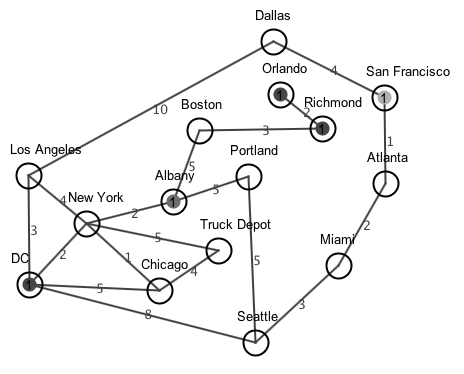
\includegraphics[scale=0.75]{map1.png}} 
\caption{\em{A sample ShippingGame map. Finally, a rational explanation for why your flight from DC to Chicago was routed through New York}}
\end{figure}\\
You control a fleet of trucks, which can pick up and deliver parcels. You can give trucks instructions at the beginning of the game.
Also, at various events, such as a truck reaching its destination, it will let you know so you can give it additional instructions.
Trucks begin the game on the Truck Depot city (there will be exactly one Truck Depot) and must return there after delivering all parcels for the game to end.

\section{3. Installation and running}
\subsection{Installation}
The code for this project is provided as a .jar file, without source files. Various data files are provided as text files in folders.
\begin{enumerate}
\item Create a new Java project in Eclipse, named A6.
\item Download ShippingGame.jar and all of the data folders and drag them into your A6 folder. Don't change the names of any of the folders or the code won't be able to find the data.
\item Right click A6 --> Build Path --> Add External Archives --> Select ShippingGame.jar and click Open.
\item Right click A6 -> Build Path --> Configure Build Path... --> Expand ShippingGame.jar by clicking on the triangle to the left of it --> Select Javadoc Location --> Click Edit... --> Select "Javadoc URL" --> Click Browse... --> Select the "doc" folder (don't expand it) and click Open, Click Ok, Click Ok.
\item Create a package called \textbf{student} in folder src (right click src --> new... -> package) . All code you write goes in package student \textbf{student}.
\item Place into package student your class MyHeap from assignment A6a. You will have to put a package statement at the top of it.
If you are not sure your MyHeap is correct, you can use one that we wrote, which will be made available 2 days after A6a is due.
\item Create a class \textbf{MyManager} in package student extends \textbf{game.Manager}. This is your manager class, and it is your main submission. You must use the name \textbf{MyManager}.
\end{enumerate}

\subsection{Running}
\begin{enumerate}
\item Select A6 -> Run As... --> Run Configurations... --> New Launch Configuration (blank page with star in top left)
\item Click Search... next to Main class --> Select game.main
\item Click run.
\item From here on out, the settings are saved, so you can simply run the project by clicking the green run button as usual.
\end{enumerate}

\subsection{Arguments}
You can provide arguments to the runner to have it do different things. All argument combinations have to start with the name of your manager. With just the manager classname provided, the game will launch in GUI mode. There are no other applicable arguments for this mode. Any other combination of arguments will launch the game in GameRunner mode instead, where the game will automatically run your manager on a sequence of maps. 

To run GameRunner on a series of seeds <seed1> <seed2> <seed3> such as $15, 12345, 907230587$, use each seed as an argument, separated by a space. (replace MyManager with the name of your Manager):
\begin{center}
MyManager 15 12345 907230587
\end{center}
To run GameRunner on a series of $n$ random seeds, use the $-r$ flag, followed by the number of random seeds to run (replace MyManager with the name of your Manager). For example, to run your manager on 10 random seeds:
\begin{center}
MyManager -r 10
\end{center}
The GameRunner mode includes the GUI to show the progression of the run games. It also prints output of the games to the console. If you would like to just see the output and not show the GUI (headless), add the $-h$ tag. Thus, either:
\begin{center}
MyManager -h 15 12345 907230587
\end{center}
or
\begin{center}
MyManager -h -r 10
\end{center}
\begin{figure}[h]
\centerline{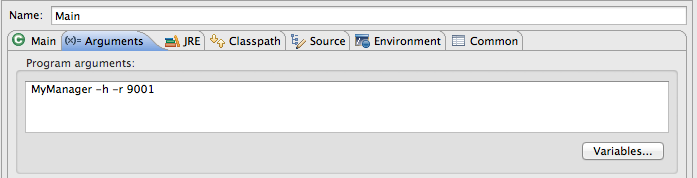
\includegraphics[scale=0.65]{args.png}} 
\caption{\em{Running MyManager in headless mode on 9001 random seeds.}}
\end{figure}

\section{4. Using the GUI}
\begin{figure}[h]
\centerline{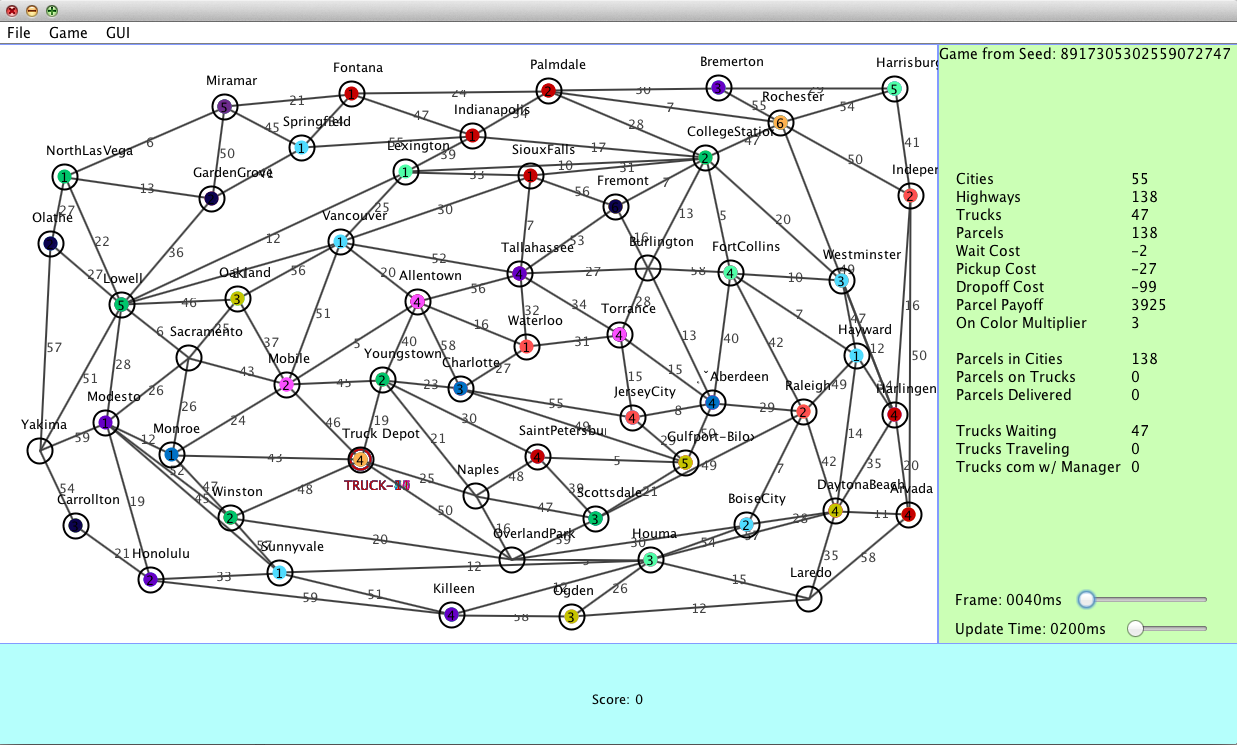
\includegraphics[scale=0.45]{gui.png}} 
\caption{\em{The Shipping Game GUI. Now with 50\% less (visual) sugar!}}
\end{figure}

Assuming the installation process went correctly and you have created a class that extends manager, you should be able to run the main class and see the gui. {\em(Note: the generated map may be different than pictured above)}. It is fully resizable. All cities (nodes) can be dragged to allow you to make the graph look cleaner, but  this purely visual change has no impact on the board state. Here are some other features.. 

\subsection{4a. Menu bar}
\begin{itemize}
\item File -> Open...: Open a JFileChooser rooted at the data/maps directory.\ You can choose a map (in JSON format) to load into the gui.
\item File -> Quit:  Close the gui and terminate the program.
\item Game -> Start: Begin the game.\ Clicking this again after the game has begun does nothing, but clicking it after the game has ended will restart it.
\item Game -> Reset : Reset the displayed game to its initial state..
\item Game -> New Random Map...: Generate a new random map with the seed (long int) given in the popup window. Exit this option by clicking cancel on the popup window.
\item Game -> Print Game JSON: Print a JSON string represention of this game to the eclipse console. Useful to save an interesting board by resetting it, printing the game JSON, and creating a new text file in the data/maps directory with the game JSON as its contents.
\item GUI -> Repaint: Repaint the gui. Try clicking this if the gui looks strange before trying other solutions.
\item GUI -> Edge Coloring: Control how edges are colored on the gui.
\begin{itemize}
\item Default: All edges are dark gray
\item Highlight-Travel: Edges being traveled by a truck are red, others are dark gray.
\item Distance Gradient: Colors edges by a linear interpolation from light to dark, based on their weights. Shorter (lighter) edges are painted in a lighter color; longer (heavier) ones are in a  darker color.
\end{itemize}
\end{itemize}

\subsection{4b. Info panel}
The panel on the right is the info panel ---it displays useful information about the currently displayed game.
The top block of data is static and will not change as the game runs.
\begin{itemize}
\item Game From...: A description of the current game ---either from seed, from file, or custom
\item Cities: Number of nodes
\item Highways : Number of edges
\item Trucks:  Number of available trucks
\item Parcels:  Total number of parcels, including delivered parcels
\item Wait Cost : Cost (per frame) of a truck doing nothing
\item Pickup Cost: Singleton cost of a truck picking up a parcel
\item Dropoff Cost: Singleton cost of a truck dropping off a parcel
\item Parcel Payoff: Singleton value of dropping off a parcel at its location
\item On Color Multiplier: Multiplier applied to the parcel payoff if the delivering truck and the parcel share a color.
\end{itemize}

The next two blocks of non-static data are changed as the game proceeds.

\begin{itemize}
\item Parcels in Cities: Number of undelivered parcels that are not on trucks
\item Parcels on Trucks: Number of undelivered parcels that are on trucks
\item Delivered Parcels: Number of delivered parcels (they have been removed from the map)
\item Trucks Waiting: Number of trucks that are currently doing nothing
\item Trucks Traveling: Number of trucks that are currently traveling an edge
\item Trucks com w/ Manager: Number of trucks that are currently communicating with the Manager —i.e. have called truckNotification(...) and are awaiting a response.
\end{itemize}

You control how often non-static data is refreshed using bottom slider Update Time. Dragging the slider to the left updates the data more often at the cost of using a tiny bit more processing 
power. For debugging purposes, it is useful to have the data update as quickly as possible, whereas once your code works correctly, you can have the data rarely updated to get the best possible score.

Finally, slider Frame controls how quickly the game progresses.\ A higher value (drag right) causes the trucks to travel more slowly and favors more computationally complex solutions, and a lower value causes the trucks to travel more quickly and favors more computationally simple solutions. It can be useful in debugging to drag the slider far to the right to watch the trucks move in slow motion. However, note that altering the slider causes the score to change and change the color of the Frame label to red. \textbf{Grading will be done at a Frame rate of 40ms, so when checking your scores make sure that you have not moved this slider} (The label will stay black when the frame rate is unaltered).

\section{5. Brief introduction to the classes}
Assuming your installation worked correctly, you should be able to see the javadoc specifications of all public classes and methods in package game.
If not, consult section 2 of this guide or ask on Piazza/at office hours.\\

The following diagram shows the class structure.\ Each interface and class in the figure is explained briefly below.\ For a more thorough explanation, see the javadoc specs.
\begin{figure}[h]
\centerline{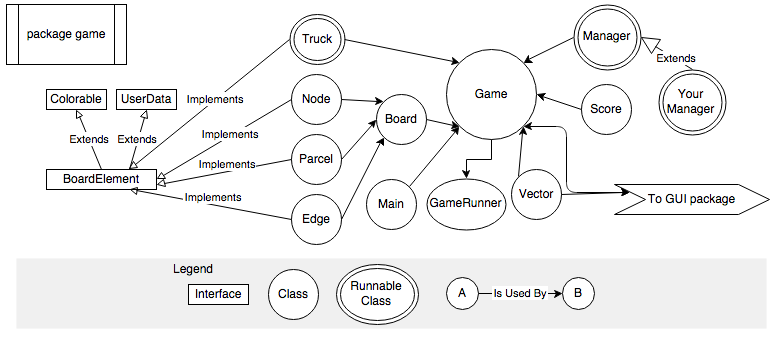
\includegraphics[scale=0.5]{hirearchy.png}} 
\caption{\em{Class Layout of package game. More lines and circles.}}
\end{figure}
\subsection{Interface Colorable}
Colorable  is implemented in classes that have a ``color''. Interface BoardElement extends Colorable, so  all elements drawn on the map have a color.
\subsection{Interface UserData}
UserData is implemented in classes that allow the user (Your manager) to store data in them. You don't have to use UserData's methods, but it may prove useful in some graph algorithms.
\subsection{Interface BoardElement}
In addition to being a catenation of the requirements of interfaces Colorable and UserData, BoardElement specifies behaviors required for displaying an object on the GUI. Implementing classes are required to be able to provide various GUI-sensitive information, such as how to draw it, what its name on the GUI is, and if there are any trucks currently ``on it``.
\subsection{Class Truck}
Instances of Truck are the game pieces of ShippingGame. Trucks take instructions from Managers and can travel the map and pick up and drop off a single parcel at a time. Trucks are runnable: each instance of Truck runs in its own thread.
\subsection{Class Node}
Each Node on the map represents a city, which is connected to other cities by highways (Edges). Nodes contain parcels until trucks pick them up. Initially, all Trucks are at the special Node TruckDepot, and they must return there before the game can end.
\subsection{Class Edge}
Instances of Edge connect the Nodes in the Board. Each Edge represents a highway that connects two cities (Nodes). Edges are undirected (bidirectional) and weighted (have length). The weight of the Edge tells how long it takes for a truck to travel a given Edge..
\subsection{Class Parcel}
Instances of Parcel are the scoring pieces of ShippingGame.\ Each Parcel starts at a city.\ It awards points when it is  delivered to its destination.\ The game can end only after all Parcels have been delivered.
\subsection{Class Board}
The Instance of Board for a game contains the Nodes, Edges, and Parcels associated with the game. It has the scoring constants related to various actions taken during the game and convenience methods such as getting a random Node or random Edge.
\subsection{Class Score}
An instance of Score encapsulates the score of the game. In addition to preventing the user (your manager) from altering the score, it has convenience methods for checking for a valid color and calculating the cost of a Truck Speed.
\subsection{Class Vector}
Vector is  similar to class Point of Java except that it uses doubles instead of ints. It is used internally for calculation and is provided as a convenience.
\subsection{Class Main}
Main begins execution of the game —it has method main. It contains static convenience methods for use all over the project.
\subsection{Abstract class Manager}
You have to extend Manager. The non-abstract behavior of class Manager gives convenience methods for getting the map, trucks, and parcels in the game. It also gives enum Notification, which specifies the different reasons a Truck would notify the Manager of a change.
\subsection{Class Game}
An instance of Game represents the game as a whole. It is the unifying factor, tying all  the other pieces together and communicating with the GUI to keep the visual version of the game up-to-date. It includes convenience methods for querying the current state of the game.
\subsection{Class GameRunner}
An instance of GameRunner provides for the automatic running of many games. This is useful to automatically test your manager on many boards, and it can be accessed via arguments given to main.
\subsection{Your Manager}
An instance of your manager fills in the missing behavior of class Manager to determine how the game runs. See the next section for more on what you have to do in your extension of class Manager.

\section{6. Your tasks}
Your primary task is write a subclass of abstract class Manager.\ You must override the two abstract methods of class Manager: \textbf{run()} and \textbf{truckNotification(...)}, which determine the behavior of the trucks in the game. On their own, trucks don't do anything; it's up to you to write code to instruct them.\ The
design of these two method is up to you. We give a few details below.\\

\begin{figure}[h]
\centerline{
\includegraphics[scale=0.35]{fry.jpg}} 
\caption{\em{The average intelligence of your shipping boys}}
\end{figure}

Procedure run() is called as soon as the game begins. In run(), you can do initial computation and give trucks their initial instructions.\ Additionally, the body of run() is executed in a separate thread from the trucks, so you can continue to do computation after the trucks have begun their travel. Your implementation can either loop forever and continually add information to the trucks or execute a single time for initial instructions and then rely on method truckNotification for further interaction.\\

Truck t calls truckNotification(Truck t, Notification message) when it does something of note, to ask for more instructions. For example, upon arrival at a new city, t may send a notification that there is a parcel at the city. Perhaps you want t to pick up that parcel before continuing on its route. For a full list of the reasons a truck would call this method, see Manager.Notification in the previous section and in the javadoc. This method is called by truck t in t's thread. 

\section{7. Concurrency}
Because every Truck the manager interacts with exists in its own thread, Shipping Game is inherently multithread. Your manager has to be able to handle several trucks calling truckNotification concurrently, without crashing or giving incorrect instructions. That said, depending on the complexity of your solution, you may not need to worry about concurrency at all. For example, consider the following pseudo-code approach to the shipping game problem.
\begin{algorithm}
\caption{Basic Preprocessing} \label{alg:ls}
\begin{algorithmic}[1]
\FOR{Parcel p}
\STATE Choose arbitrary truck $t$ to deliver $p$. Store $p$ in a data structure in $t$'s user data.
\ENDFOR
\end{algorithmic}
\end{algorithm}
\begin{algorithm}
\caption{Basic Truck Notification ($t$)} \label{alg:ls}
\begin{algorithmic}[1]
\IF{Basic Preprocessing not done}
\STATE Return      // It's best always to start with this if-statement
\ENDIF
\IF{there is an Undelivered Parcel in game}
\IF{$t$ holding a parcel}
\STATE Route $t$ to the parcel's destination, then drop off the parcel
\ELSE
\STATE find the next parcel assigned to $t$, route to that parcel.
\ENDIF
\ELSE
\STATE Route $t$ home
\ENDIF
\end{algorithmic}
\end{algorithm}
\\

This algorithm makes use of every truck, but because no data structure is accessed by several trucks and all internal data structures are guaranteed to be thread-safe, there is no need for worry about concurrency. Assuming no errors, a correctly implemented version of this algorithm  would probably get at minimum a good grade, likely higher.\\

If, however, you're shooting for a perfect grade, you may have to do some amount of work to ensure that your complex network of information sharing between trucks remains thread safe. Concurrent modifications of most data structures cause incorrect states, usually leading to null pointers or array-index-out-of-bound errors. Failure to write thread safe code might lead to unpredictable and catastrophic errors.\\
\begin{figure}[h]
\centerline{
\includegraphics[scale=0.45]{collision.png}} 
\caption{\em{Don't rely on Spongebob to keep your code thread safe.}}
\end{figure}

In this vein, you have a few different options to keep code thread-safe. The more powerful the tool, however, the greater the possibility of creating new and more difficult problems. Ideally, come up with a strategy, than pick the least-comprehensive tool that gives you just enough capability to prevent potential thread safety problems.
\subsection{Approaches to Concurrency}
\begin{itemize}
\item \textbf{wait() and notify()} - Power: medium. Possibility for Error: very high.\\
Java's built-in concurrency system. Threads can cause themselves to wait, using any object as a key, and wake up other threads waiting on a given object. Working out a system of wait() and notify() calls that correctly limits thread movement is difficult. At the end of the day, some higher level systems are able to accomplish the same tasks in a much safer way. Don't use wait/notify unless you really want to get your hands dirty.
\item \textbf{Synchronized Collections} - Power: low. Possibility for error: none. \\
Class java.util.Collections \href{http://docs.oracle.com/javase/7/docs/api/java/util/Collections.html\#synchronizedCollection(java.util.Collection)}{({\color{blue}\underline{API}})} provides the ability to create a synchronized collection (a synchronized set, list, map, etc...). These collections are inherently thread-safe for basic operations, including adding elements, removing elements, getting elements, and checking the size of the collection. Notably, you can't iterate over a synchronized collection without a synchronized block (see next section), so complex operations that require iterating aren't safe. If you can get away with just using Synchronized Collections, you should do so and won't have any problems.
\item \textbf{Synchronized Blocks} - Power: medium. Possibility for Error: low.\\
A synchronized block limits one thread to executing its body at a time. Other threads wait on before the statement until the executing thread finishes the block. Moreover, each synchronized block is called on some object in the form:
\begin{lstlisting}[frame=single]
synchronized(obj){
//...Do things that only one thread should be doing.
}
\end{lstlisting}
And, only one thread can access any synchronized block that is associated with that object at a time. This means that two synchronized blocks with the same object:\\
\begin{lstlisting}[frame=single]
synchronized(obj){
processA();
}
synchronized(obj){ //Note - synchronized on same obj
processB();
}
\end{lstlisting}
could not execute processA() and processB()  concurrently, because a thread's presence in one of the two blocks prevents other threads from being in either of the two blocks.\\

The simplest way to use synchronized blocks on Synchronized collections to allow iteration \href{http://docs.oracle.com/javase/7/docs/api/java/util/Collections.html\#synchronizedCollection(java.util.Collection)}{({\color{blue}\underline{See API}})}. That way only one complex (iterative) process can occur on the collection at a time, and nothing can go wrong. \textbf{This combination is probably the best solution for this project, and should be considered first}.
\item \textbf{Locks and Locking} - Power: High. Possibility for Error: High\\
Locks (and Semaphores and other equivalent classes) take the two pieces of a synchronized block ---preventing other threads from accessing code and letting other threads know that the going is clear--- and separate them into two individual lines of code. Only one thread can "own" a mutex (mutual exclusion object) at a time (semaphores are generalized to allow N threads), so when a thread acquires a Lock l, all other threads that attempt to call l.lock() are forced to wait until the thread that owns the lock calls l.unlock(), at which point an arbitrarily chosen thread that is waiting will call l.lock() and proceed. This gives you ultimate control over which threads execute what where and when, but it is  prone to issues such as deadlock in which two threads are each waiting to acquire a lock owned by the other. Locks and Semaphores are overkill for all but the most complex solutions and are most likely not necessary for this project. 
\end{itemize}

\section{8. What to hand in when}
This project is due on the last day of class, \textbf{Thursday, 4 December, at 11:59PM}.
Submit on the CMS a zip file that contains all the java file in package student ---these are the ones you wrote.
This includes you class MyHeap.
\\



\end{document}